\formdesc{La quantification}

unipolaire : $q = \cfrac{Dyn}{2^n} [V]$

bipolaire : $q = \cfrac{2Dyn}{2^n} [V]$

$Code = \cfrac{U_{in}}{q} [-]$ division entière

$Xq = Code \cdot q [V]$

L’erreur de quanti. est bornée entre -q/2 et +q/2

\hformbar

\formdesc{Echantillonage}


Si pleine gamme dynamique avec sinus : 

$SNRQ = 6.02N + 10.8 + 20log(\cfrac{V_{rms}}{2U_{ref}}) $

$\Delta SNRQ = SNRQ1 - SNRQ2 =10log(N_{OSR}) $


Tension efficace du bruit de quantification : 

$\sigma_{nQ} = \cfrac{Vref}{2^{n-1}\cdot\sqrt{12}}$

Densité spectrale de puissance :

$S(f) = k_Q^2 = \cfrac{\sigma_{nQ^2}}{FS} = \cfrac{q^2}{12FS} [V^2 / Hz] $

Rapport signal sur bruit de quantification :

$S(f) = 10log(\cfrac{\sigma_{x}^2}{\sigma_{nQ}^2})  = 20$


Si surechantillonage  ajout d'un filtre et d'un OSR
\vspace{5mm}

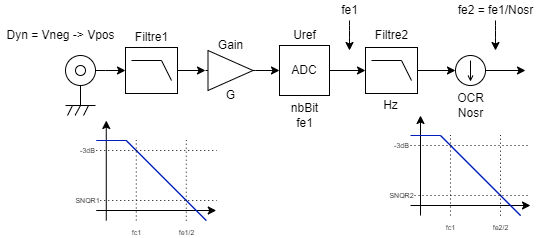
\includegraphics[width = 0.49\textwidth,center]{img/Chaine-aquis.drawio.png}
